%!TEX root = ../main.tex
\chapter{Energy Scale Calibration of the AHCAL}
\label{chap:ECalibAHCAL}

The CALICE Analog Hadronic Calorimeter (AHCAL) technological prototype was installed at the SPS CERN facilities in July and August 2015, in order to provide energy and time measurements of electromagnetic and hadronic showers using plastic scintillators. The data recorded in each cell of the calorimeter is measured in ADC counts. Due to difference in light yield and gain, this scale cannot be compared directly between different channels. Therefore to compare them, all channels have to be scaled to a common physical energy unit. For the AHCAL, the Minimum Ionizing Particle or MIP unit is chosen. This unit relates to the cell energy in a well understood physical process almost independent of outside conditions.

The conversion requires a calibration of each cell of the calorimeter which is by itself a challenge due to the high number of readout channels. In this testbeam, 3744 channels had to be calibrated. Due to the boards equipped with various types of SiPMs, the procedure needs to be automatic and robust to extract the calibration constant for each channel. At the end, all the calibration constants are entered in the official CALICE database.

This chapter will describe the procedure performed for the AHCAL energy scale calibration. In this chapter, only the calibration of the energy scale of the detector was performed. A dedicated analysis of the performance of the detector focused on energy is being finalized \cite{AmbraEnergy, AmbraTokyo}.

\section{Energy Calibration of the AHCAL}

Every channel of the detector provides a measure of the energy deposited in ADC units. To compare them or combine them, all channels need to be normalized to a common physics scale. The AHCAL uses muons to provide the calibration to the common scale as Minimum Ionizing Particles or MIP. Therefore muon runs were recorded. As detailed in section \ref{sec:PartInter}, the energy deposited in a single AHCAL cell follows approximatively a Landau distribution but due to the electronic noise, the resulting response is convoluted with a Gaussian distribution. The maximum of the Laudau-Gaussian convolution density function is defined as the MIP constant ($M_{i}$) for the i-th channel. The conversion to the MIP energy scale for a AHCAL cell is expressed as:
\begin{equation}
	E_i = \frac{(A_i - P_i) \times IC_i }{\frac{M_{i}}{ICP_i}}
\end{equation}

where $E_i$ is the calibrated amplitude in MIP, $A_i$ the measured amplitude in ADC, $P_i$ the pedestal in ADC, $ICP_i$ the intercalibration between calibration and physics mode, $IC_i$ the intercalibration between High/Low gain (equal to 1 in case of HG measurement) and $M_{i}$ the MIP constant of the i-th channel in $\frac{ADC}{MIP}$. In case of correction for SiPM saturation, the following formula is used
\begin{equation}
	E_i = \frac{f^{i}_{unsat}( (A_i - P_i) \times \frac{IC_i \times ICP_i}{G_i} )}{LY_{i}}
\end{equation}

where $f^{i}_{unsat}$ is the inversed of the SiPM saturation function and $LY_{i} = \frac{M_{i}}{G_i}$ the light yield of the i-th channel.

\subsection{Pedestal extraction}

To obtain the correct MIP constant, a pedestal subtraction has to be done. The pedestal value for each channel is extracted from the data taking muon runs. In order to be consistent, the pedestal value is extracted in the same running mode as data taking .i.e in auto-trigger (AT) \cite{Hermberg:2015gaa}. For each channel and memory cell, a histogram is filled with the ADC value of a cycle in case no Hit Bit is set for the channel. The extraction is performed in an iterative way due to a high energy tail that is not yet understood and could come from inefficiency in the trigger.

\begin{figure}[htbp!]
	\centering
	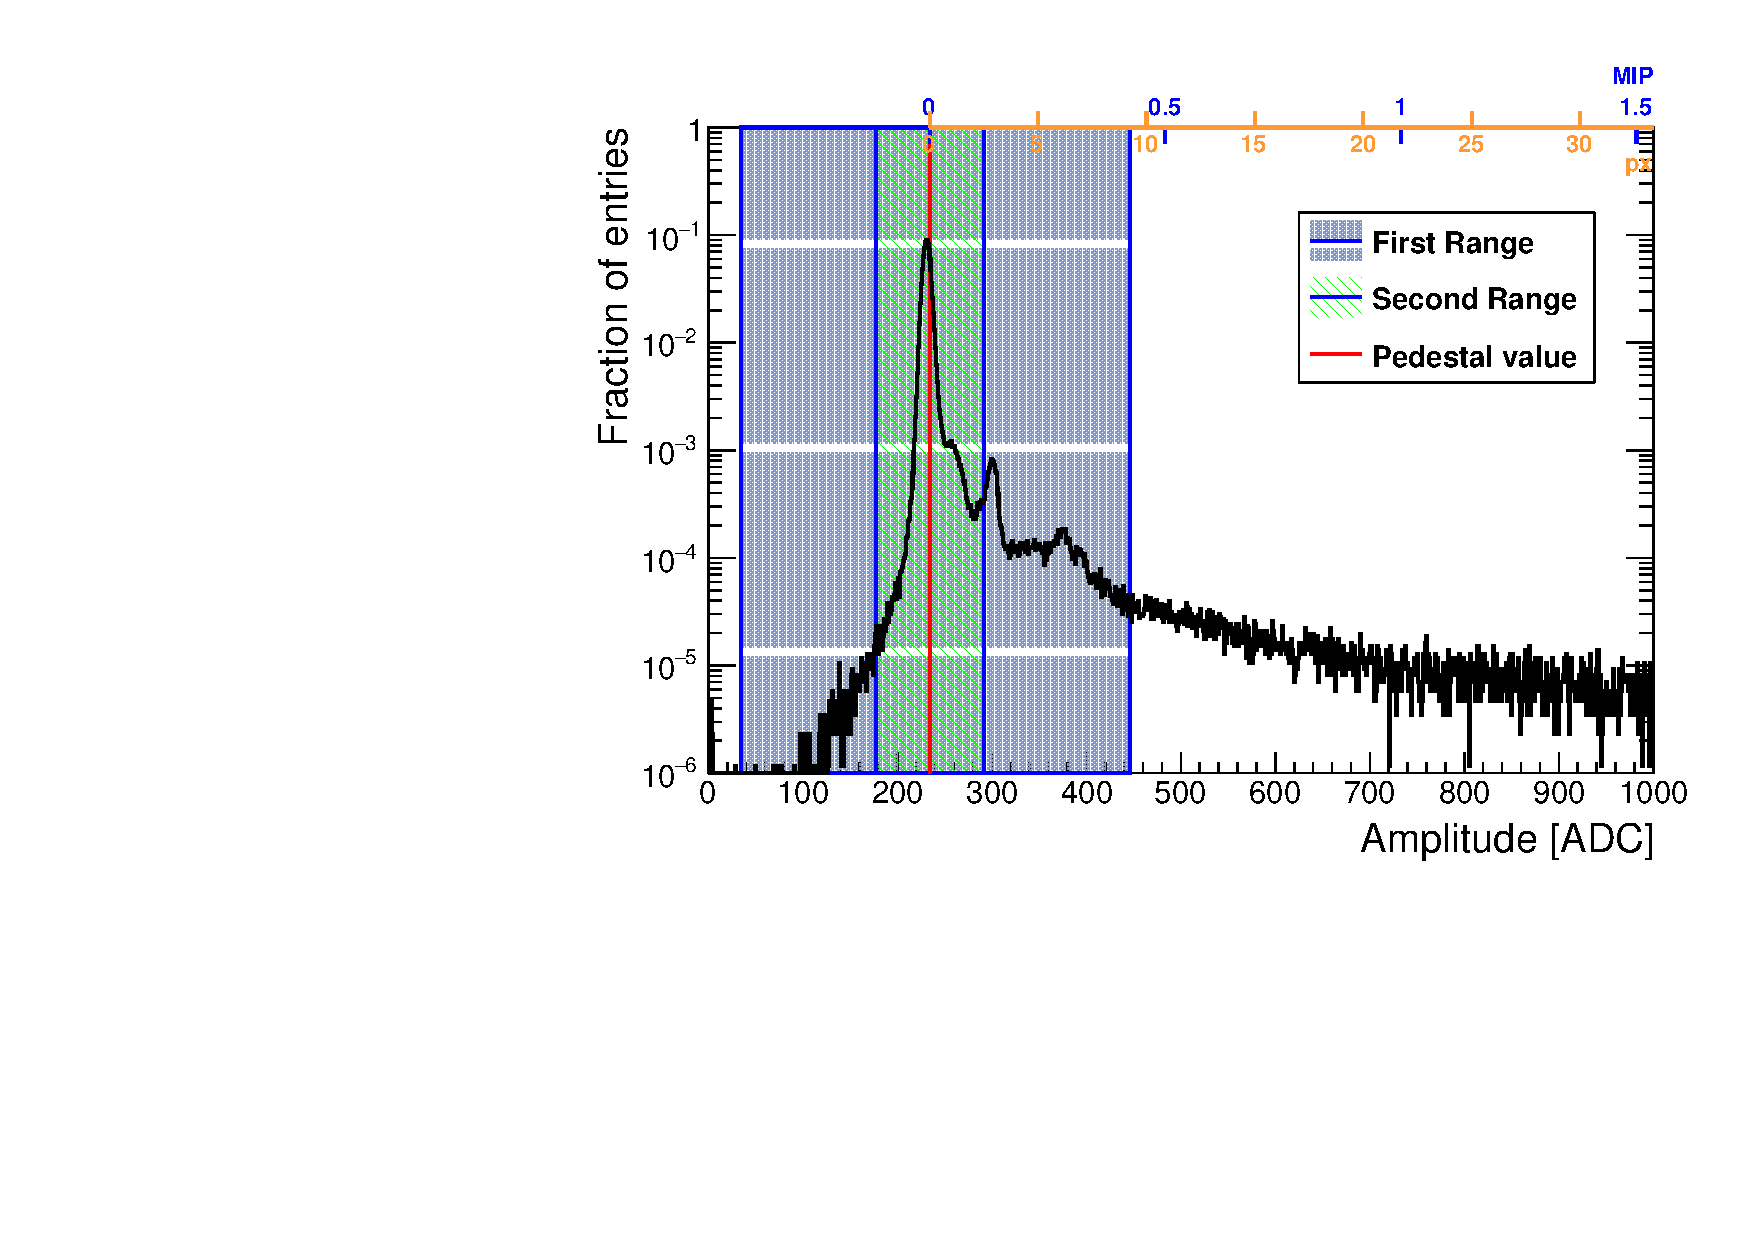
\includegraphics[width=0.7\linewidth]{../Thesis_Plots/EnergyCalib/Plots/PedestalExtractionExample.pdf}
	\caption{Typical pedestal distribution of a channel in auto-trigger mode. The different colored boxed represent the iterative procedure to extract the pedestal value marked with the red line.} \label{fig:PedExtraction}
\end{figure}

As the SiPM noise needs to be taken into account for the pedestal value and considering a Poisson statistic, one to three pixels could be fired due to DCR and cross-talk. The fitting range then needs to be in the same order of magnitude of 1 to 3 pixels. For this, the histogram range is reduced in the range of 3 RMS around the mean. It is done iteratively two times. Then the mean of the histogram is taken the pedestal value as shown in figure \ref{fig:PedExtraction}. As no pedestal subtraction memory cell-wise is performed in the reconstruction at the moment and the database structure is not designed to have the pedestal constant for each memory cell, a mean over all memory cells is computed per channel. The difference between the mean pedestal and the memory cell wise pedestal shown in figure \ref{fig:CompMeanMem}. The RMS of the distribution is around 21 ADC which would correspond to an error of about 4\% on the MIP constant (assuming a typical MIP value of 500 ADC). This error is dominating in the MIP constant uncertainty.

\begin{figure}[htbp!]
	\centering
	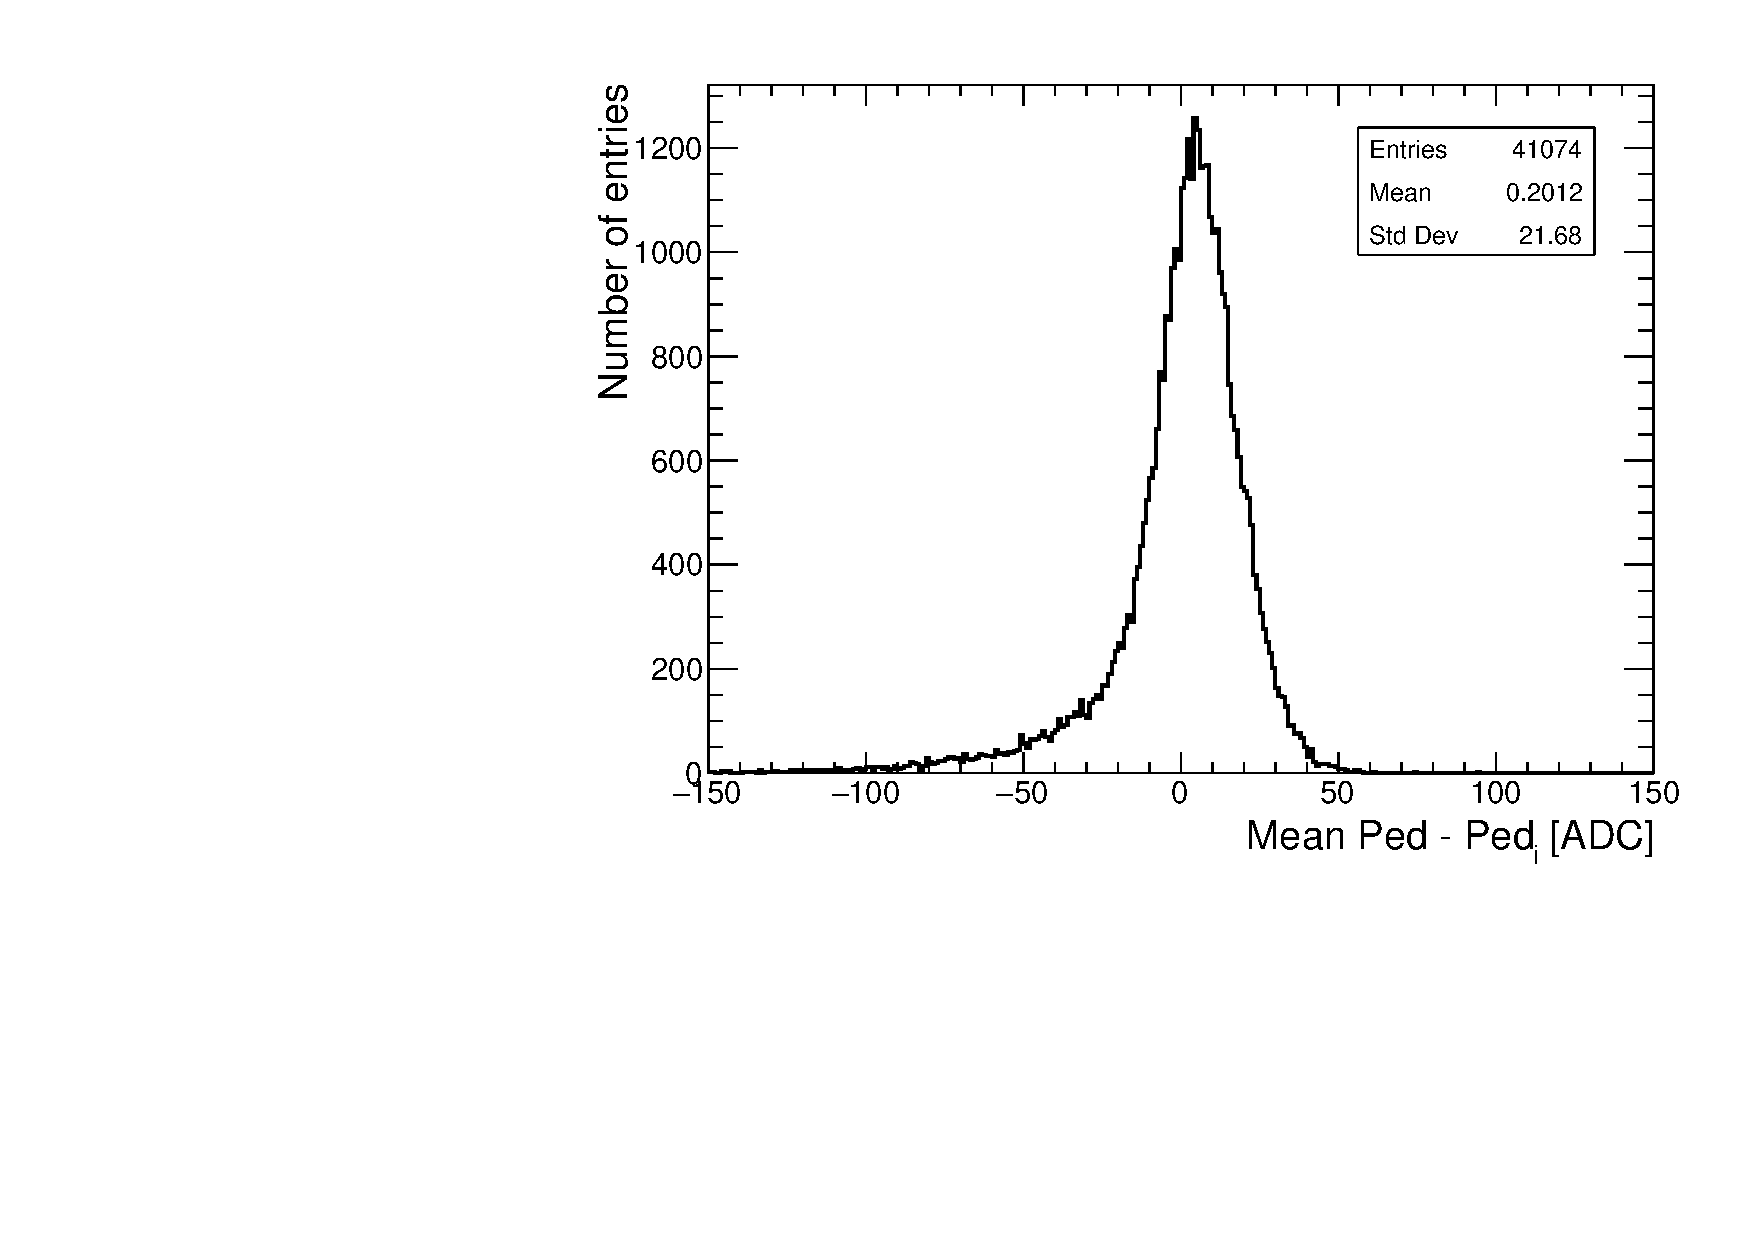
\includegraphics[width=0.7\linewidth]{../Thesis_Plots/EnergyCalib/Plots/ComparisonMeanPedtoMemorycell.pdf}
	\caption{Distribution of the difference between the mean pedestal to the memory-cell wise pedestal per channel.} \label{fig:CompMeanMem}
\end{figure}

\subsection{MIP extraction}

After the pedestal calibration, the extraction of the MIP constant for each channel can be performed. As the detector was equipped with various types of SiPM and boards designs, the extraction procedure needed to be automatized and robust. In order to reduce noise in the energy spectra of each cell that would lead to unstable fits and wrong MIP constants, a simple track selection has been performed as explained in section \ref{subsec:Muon_sel}.

After the selection, a histogram for each channel is filled with the energy value of each hit in ADC which are already pedestal subtracted memory-cell wise. Then the fitting procedure is performed. The fitting procedure is very sensitive to the initial parameters of the fit and can be quite difficult with the variety of SiPM and tiles in the AHCAL. To ensure a good fit, an iterative fitting procedure is performed. Only channels with more than 1000 entries are considered. The detailed fitting procedure is explained in \cite{FabianThesis}. The parameters to fit are: the area or normalization constant $A$, the width of the convoluted Gaussian $\sigma_G$, the MPV of the Landau distribution $MPV$ and the width of the Landau distribution $\sigma_L$

First, the area $A$ of the histogram is fitted with $\sigma_G$, $MPV$ and $\sigma_L$ fixed. Secondly, the parameters $\sigma_G$, $MPV$ and $\sigma_L$ are released and fitted as well. Finally, a final fit is performed on the four parameters in the range in the range of 30\% of the maximum of the previous fitted function. This procedure was adapted to accommodate for the high number of channel to be fitted. The procedure can be done in parallel for each layers in the detector. In an additional step, a histogram for each channel is filled with the energy value of each hit in ADC with a cut at 0.5 MIP of the previously extracted $MPV$ if available and the fitting procedure is iterated. The difference of the extracted $MPV$ value without the iteration is around 1\% which is within the uncertainty on the MIP value. But the iteration can, in some cases, recover some bad fitted channels. A typical example of a MIP fit can be seen in figure \ref{fig:MIPFit}.

\begin{figure}[htbp!]
	\centering
	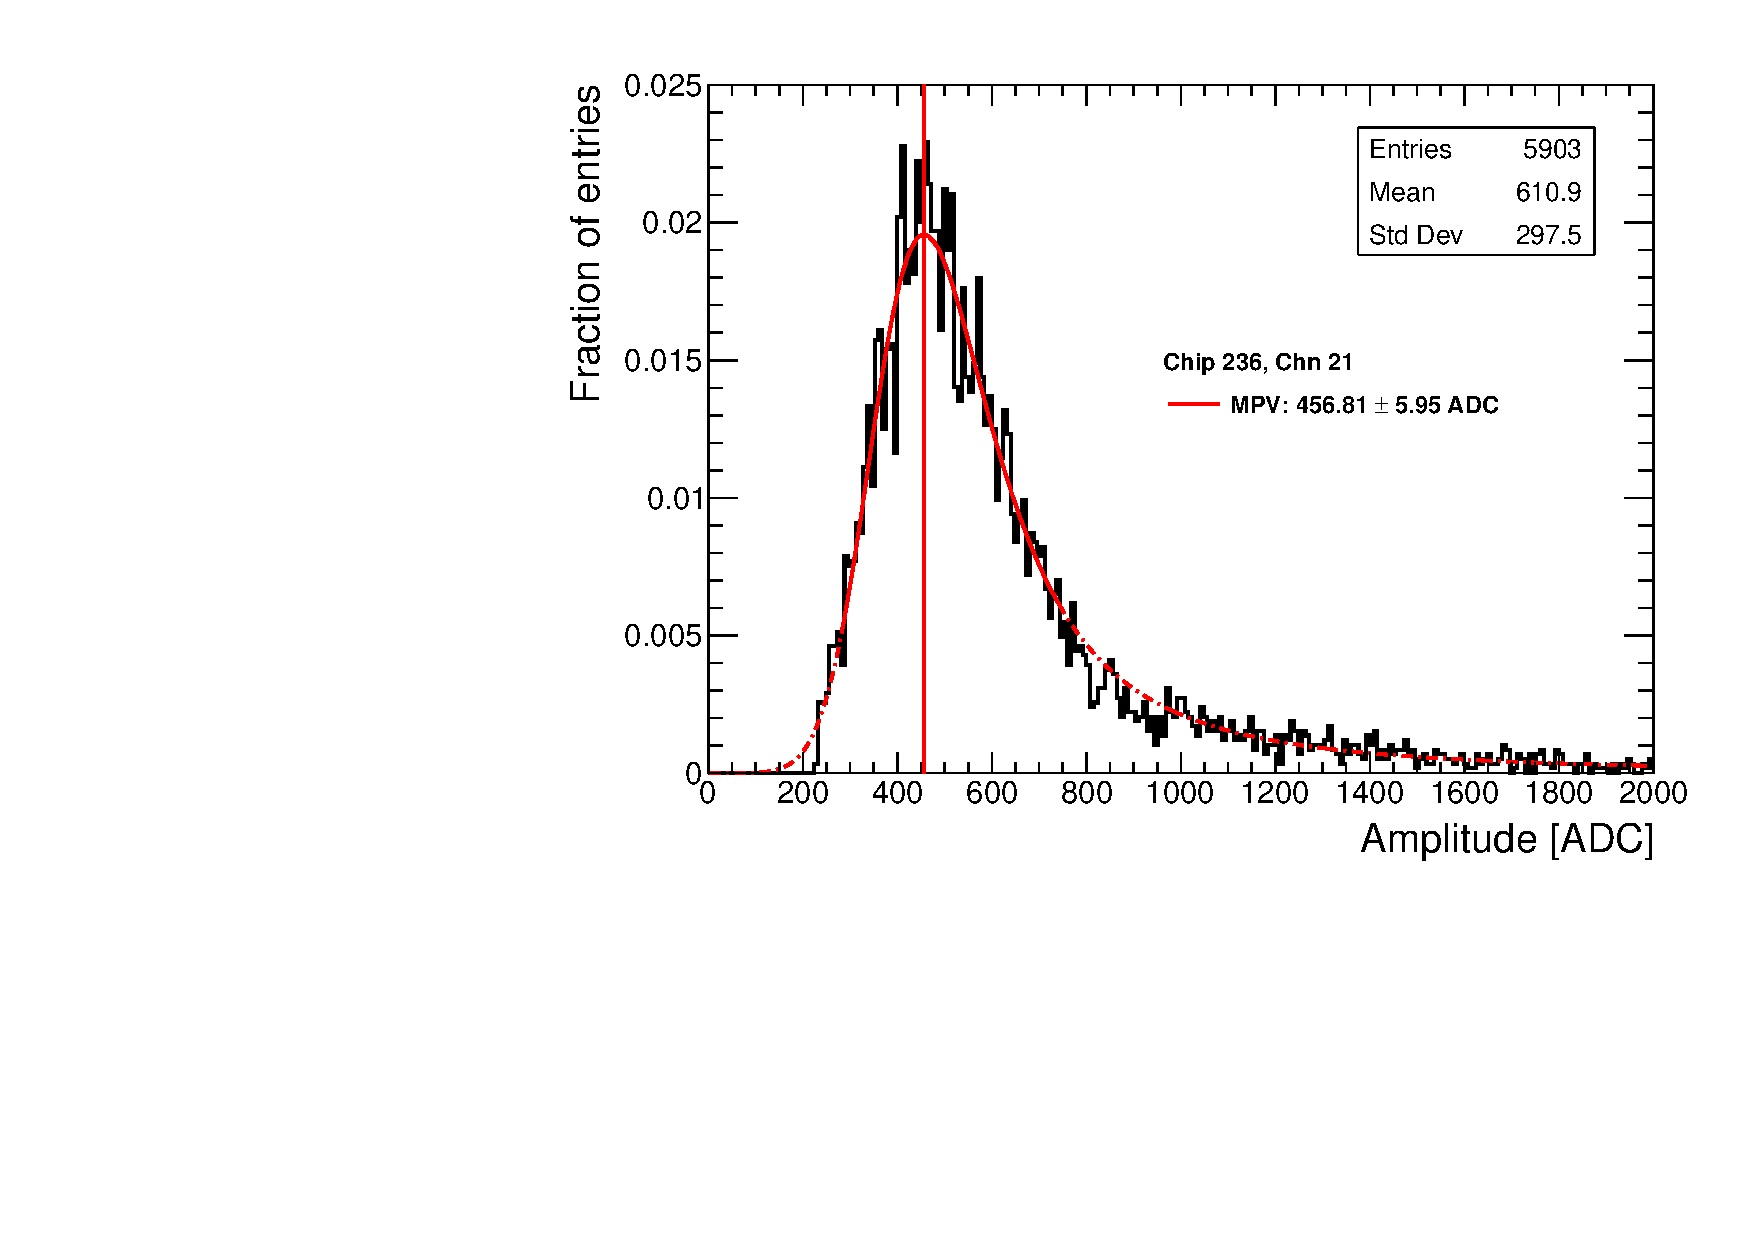
\includegraphics[width=0.7\linewidth]{../Thesis_Plots/EnergyCalib/Plots/ExampleMIP_Module3.pdf}
	\caption{Typical energy distribution in a single channel of the AHCAL with the data collected in July 2015 at CERN.} \label{fig:MIPFit}
\end{figure}

In this way, for the testbeam in July 2015, 72\% of the channels are fitted (over 3744 channels). This does not mean that 28\% of channels are dead as for the most part, the outer channels (on the border of the HBUs) of the layers 11 to 14 don't have enough statistic to perform a fit. In order to have a value for the outer channels, especially for the layers 11 to 14, the values are combined with previous testbeams performed in April and May 2015 with these layers. Finally, if a channel is does not have a value, the mean and mean error of the MPV distribution of a chip or layer is used. In this way, all 3744 channels have a MIP constant. Excluding dead and noisy channels (see appendix \ref{appendix:deadChn}) which account for 15\% of the channels, 3171 channels have been calibrated.

\section{Calibration Results}

In this section, a small assessment of the performance of the detector calibration is performed.

\subsection{MIP extraction results}

The results of the MIP extraction are shown in table \ref{table:MIPAHCAL} and are regrouped by SiPM types. The results are well compatible with \cite{SarahMaster} although there is slight difference in the number of fitted channels that may come from the differences in our method and also that, in this table, all dead and noisy channels are rejected.

\begin{table}[htb!]
	\centering
	\caption{Table containing the results of the MIP extraction. The results are regrouped by SiPM type. Dead and noisy channels are rejected.}
	\label{table:MIPAHCAL}
	\begin{tabular}{@{} cccc @{}}
		\hline
		Layer \# & MPV [ADC] & RMS [ADC] & $N_{fitted}$\\
		\hline
		\hline
		1-2 & 66.72 & 35.54 & 172\\
		3 & 501.71 & 50.4 & 142\\
		4-5 & 796.54 & 113.12 & 265\\
		6-10 & 250.99 & 62.72 & 414\\
		11-12 & 285.85 & 62.83 & 1069\\
		13-14 & 307.73 & 58.96 & 1109\\
		\hline
	\end{tabular}
\end{table}

\subsection{Error of the calibration procedure}

After the calibration, it is necessary to evaluate the performance of the calibration procedure by looking at the relative error on the extracted MPV value for a MIP. The figure \ref{fig:MIPError} shows the relative error $\frac{\Delta MIP_i}{MIP_i}$ computed for all the channels of the detector. The relative error on the MIP value is for most of the channels in the expected range of 1 to 3\% and compatible with previous results \cite{SarahMaster}. Some higher values can be seen, this comes from the EBU where difficulties were met due to high noise.

\begin{figure}[htbp!]
	\centering
	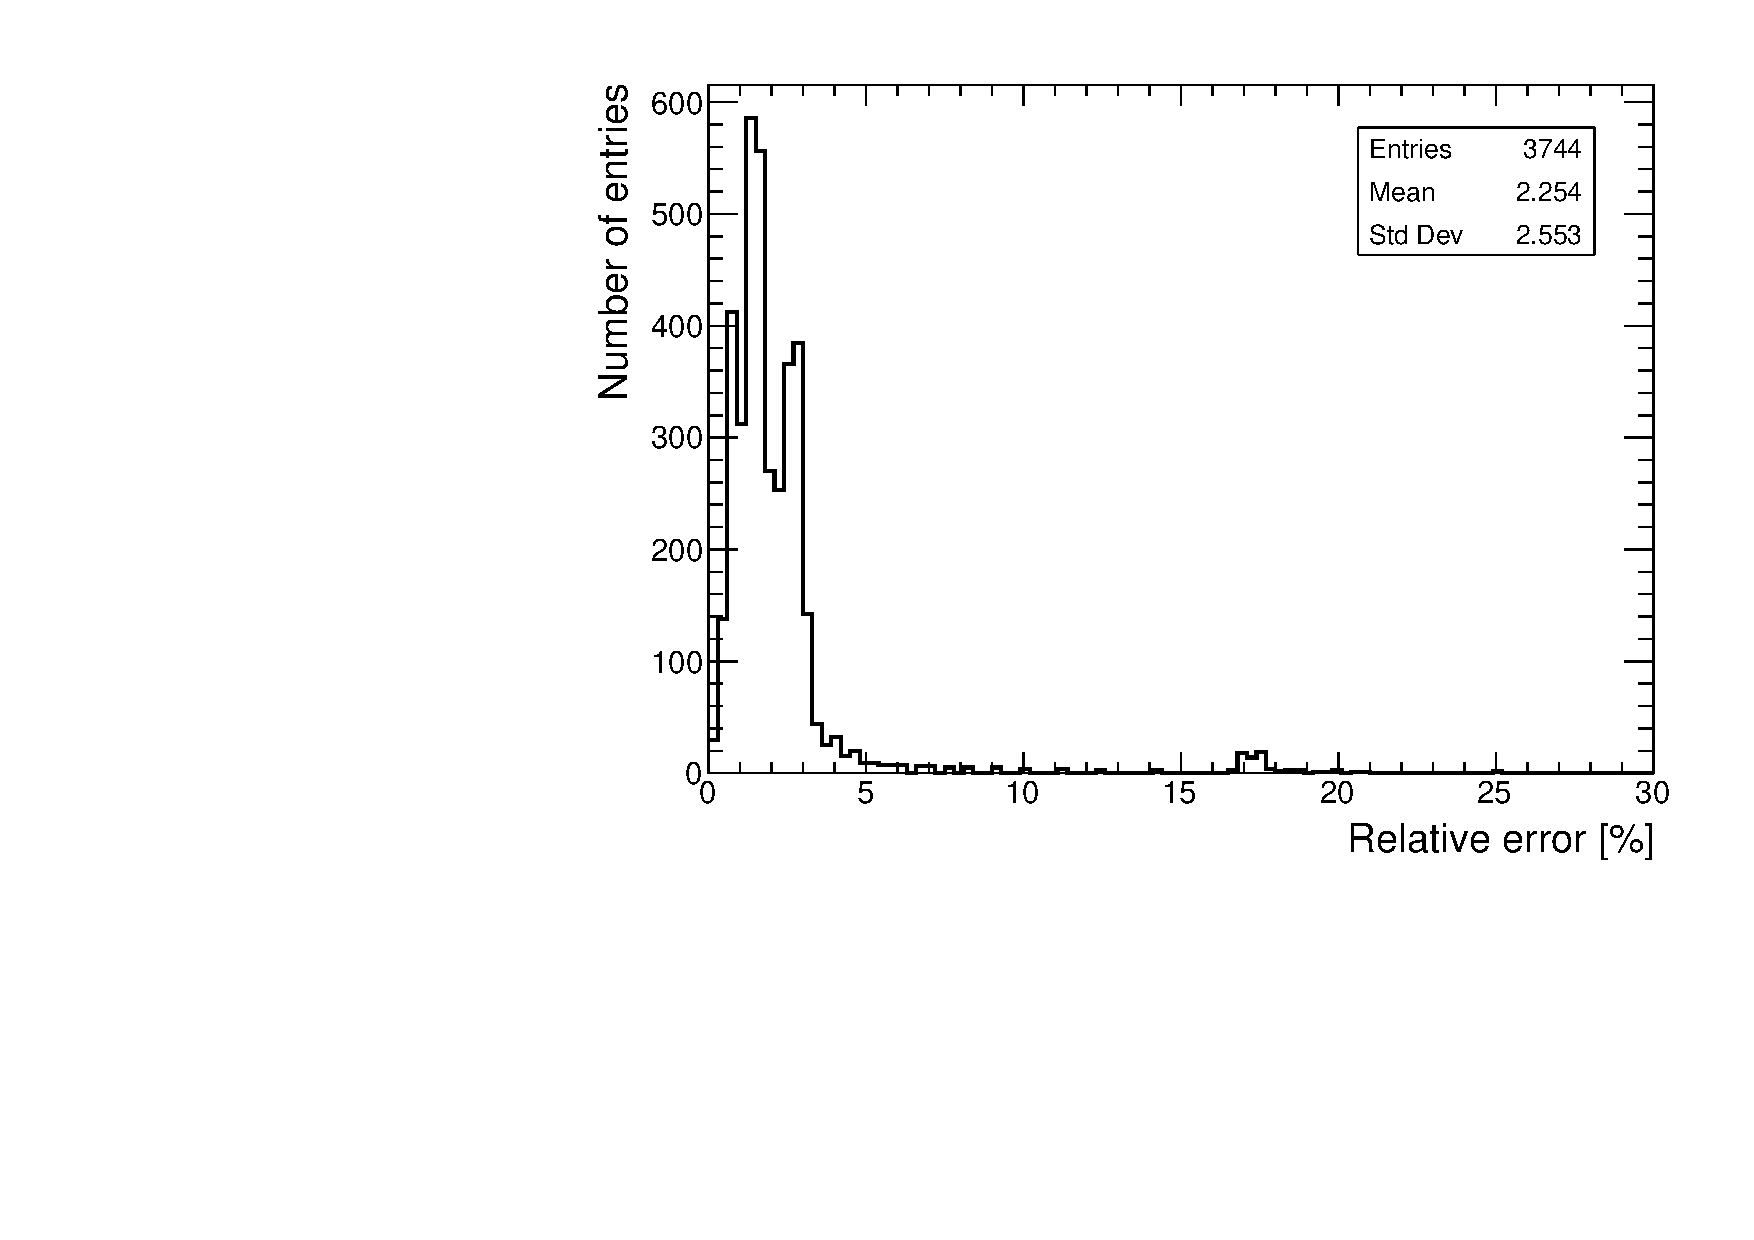
\includegraphics[width=0.7\linewidth]{../Thesis_Plots/EnergyCalib/Plots/RelativeErrorMIP_Combined.pdf}
	\caption{Relative error of the MIP value extracted.} \label{fig:MIPError}
\end{figure}

\subsection{Comparison with simulation}

The MIP calibration defines the energy scale for measuring energy depositions in the AHCAL. It is needed to carefully calibrate and validate the MIP calibration in data and simulation in order to get comparable results. Applying the MIP selection, it results in energy depositions of single MIP amplitudes for all channels. The comparison of the MIP spectrum for the whole AHCAL between data and simulation in figure \ref{fig:MIPData_MC} shows that the shape of the hit energy spectrum matches relatively well. The data appears slightly wider than for simulation as channel-wise mis-calibrations are not modeled in the simulation. This comparison validates the digitization of scintillator-SiPM readout calorimeters.

\begin{figure}[htbp!]
	\begin{subfigure}[t]{0.5\textwidth}
		\centering
		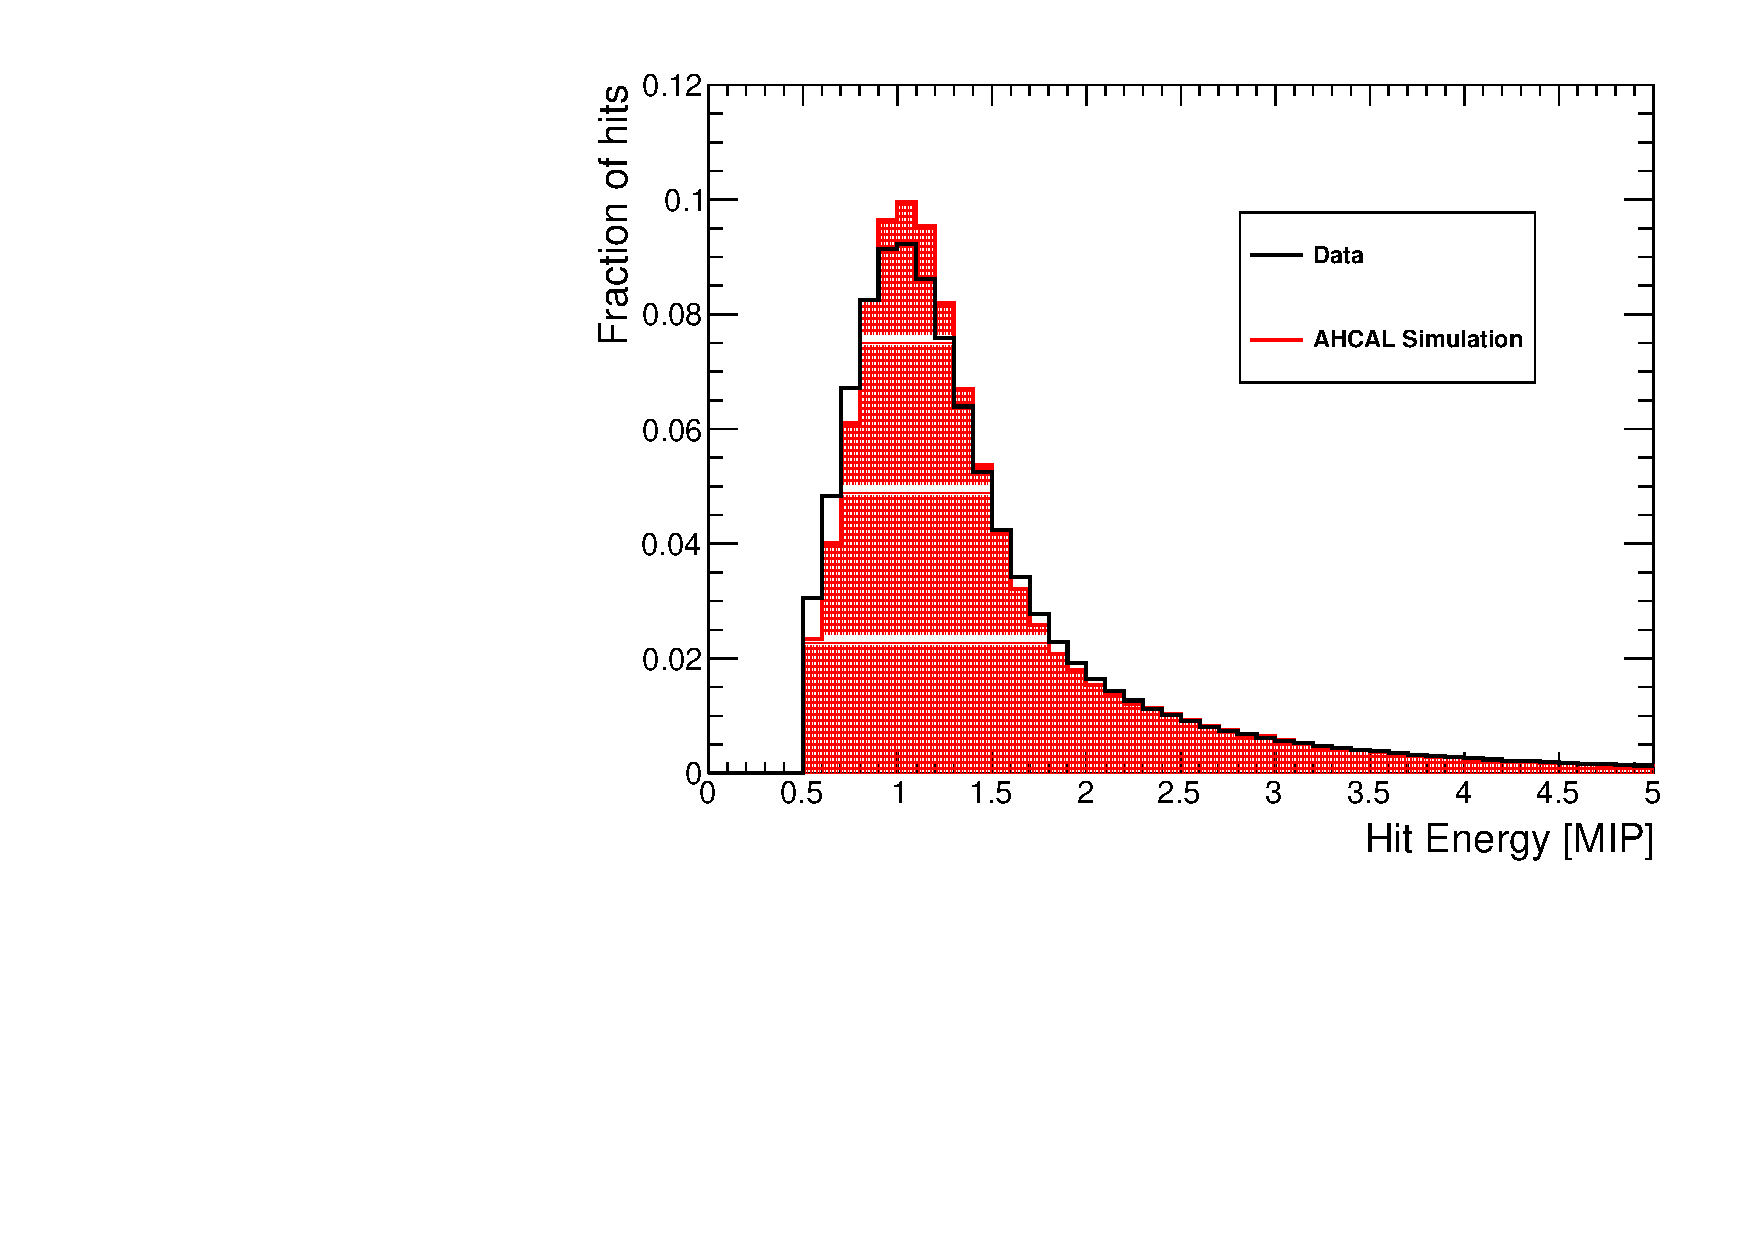
\includegraphics[width=1\linewidth]{../Thesis_Plots/EnergyCalib/Plots/ComparisonMCData_MIPPeak.pdf}
		\caption{} \label{fig:MIPData_MC}
	\end{subfigure}
	\hfill
	\begin{subfigure}[t]{0.5\textwidth}
		\centering
		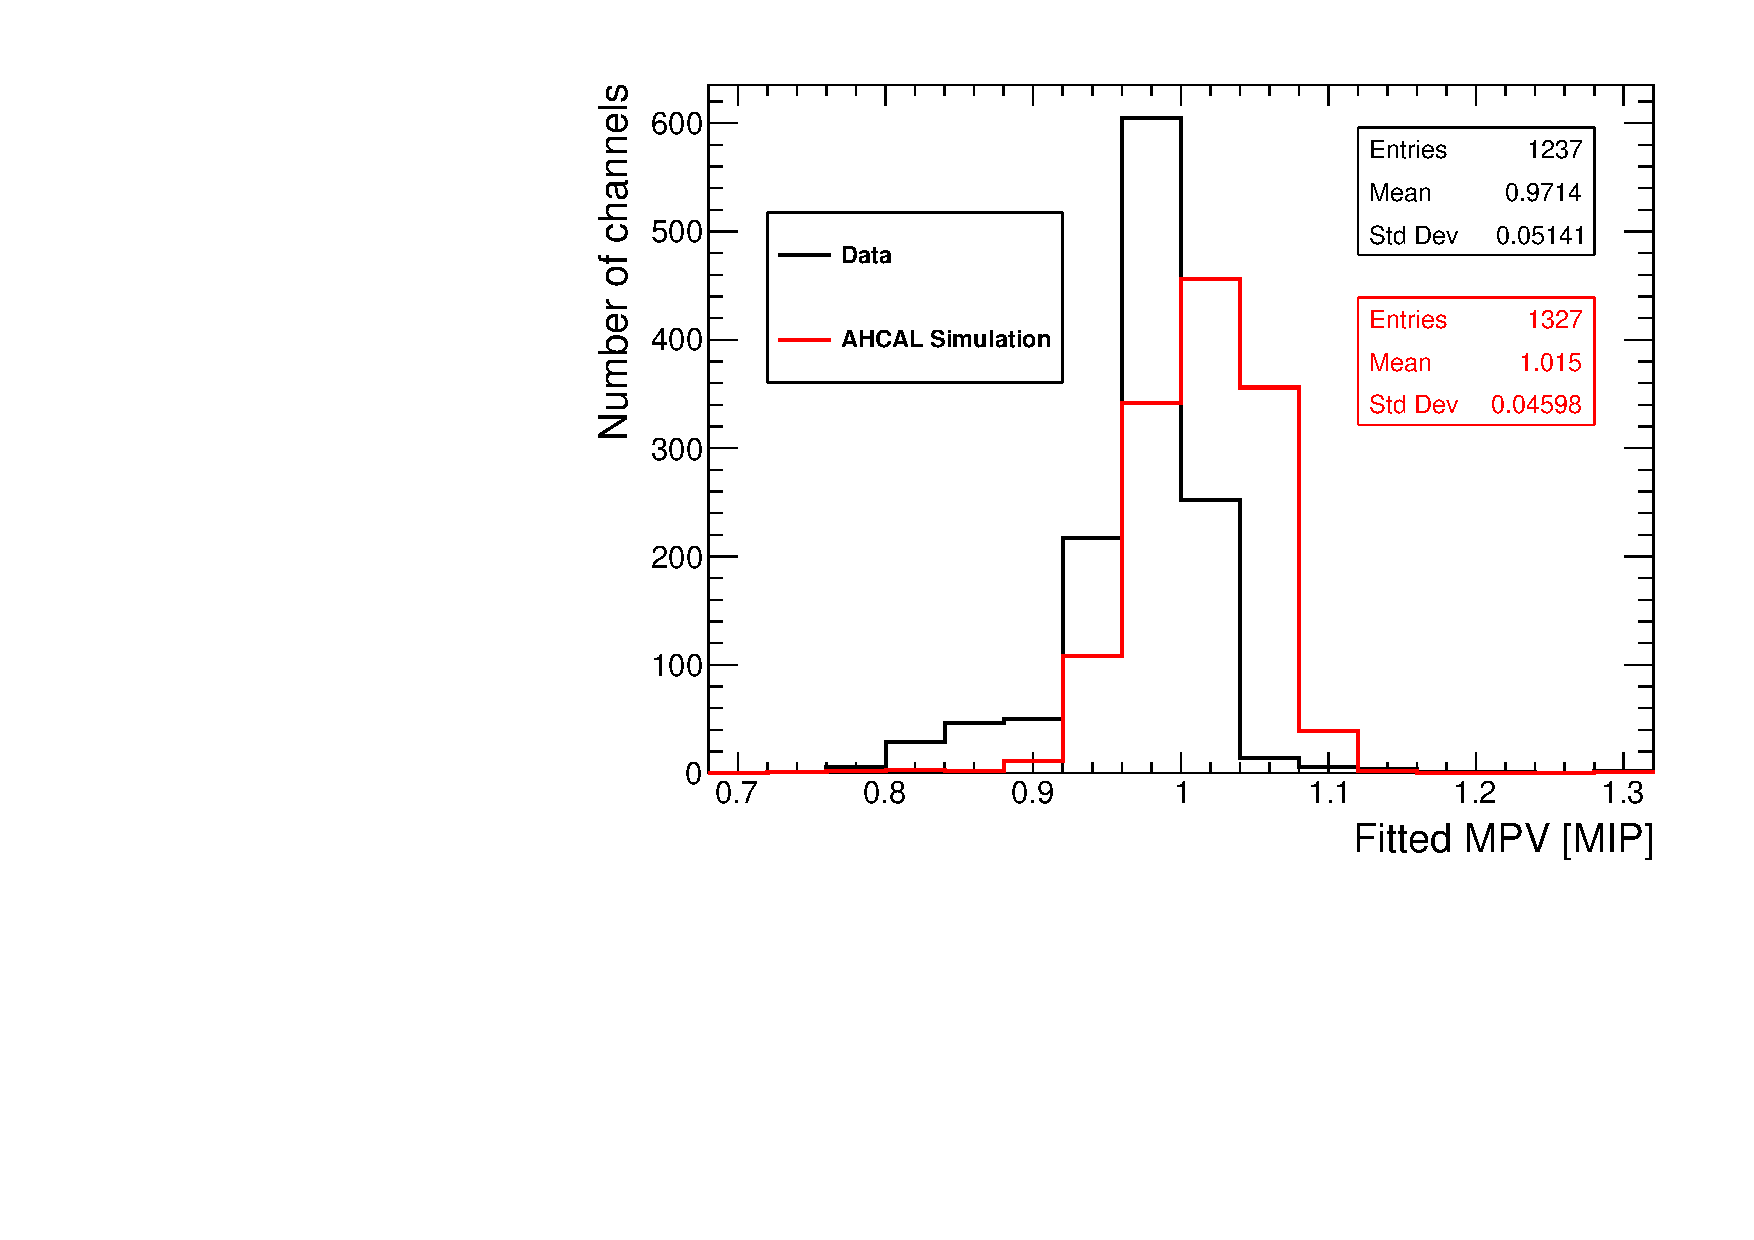
\includegraphics[width=1\linewidth]{../Thesis_Plots/EnergyCalib/Plots/ComparisonMCData_MPV.pdf}
		\caption{} \label{fig:MPVData_MC}
	\end{subfigure}
	\caption{\subref{fig:MIPData_MC}) Hit Energy Spectra for the complete AHCAL for muon like-track hits in the data of July 2015. \subref{fig:MPVData_MC}) Distribution of fitted MPV in single channels of the AHCAL.}
\end{figure}

The extraction of the MPV value in data and simulation has been done for each single channels of the AHCAL. The figure \ref{fig:MPVData_MC} shows the obtained distribution. Ideally, the fitted MPV should peak at the unity for all channels. But in practice, due to the fitting procedure, mis-calibrations and statistic limitation, this results in a widening of the distribution. Both data and simulation give a mean value around 1 MIP for the AHCAL indicating a good average calibration at the cell level. The higher values to the right that appear in the data have been checked and all channels present a good fit. The AHCAL simulation is slightly shifted to the right to higher values but still reasonably close to unity.

\subsection{Systematic on the MIP scale}

A systematic error on the MIP scale can be derived by dividing the muon sample of the July 2015 data into two sub-samples by even or odd run number. This will take into account not only the error on the MIP calibration but as well variations due to temperature or temporal variations. Then each sample is fitted using the same fitting procedure as described above.

\begin{figure}[htbp!]
	\centering
	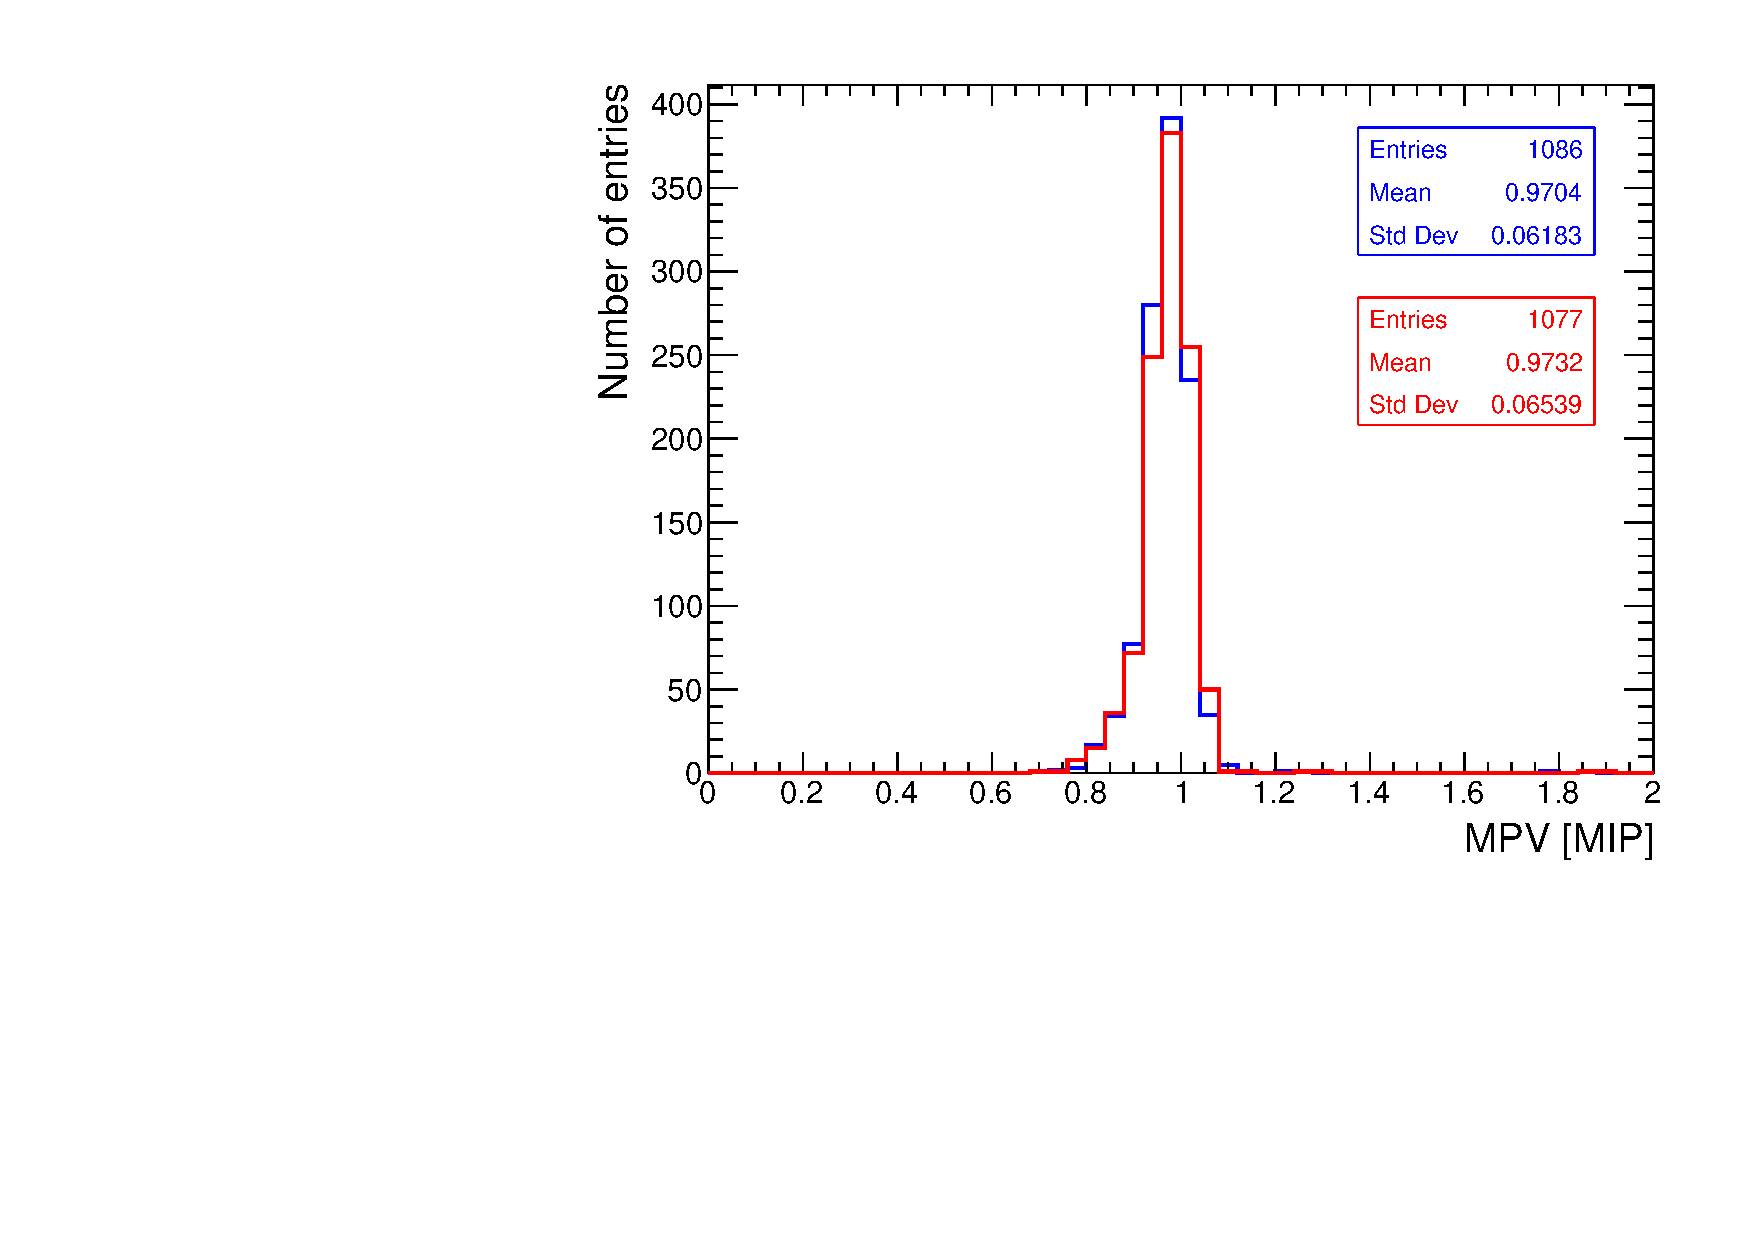
\includegraphics[width=0.7\linewidth]{../Thesis_Plots/EnergyCalib/Plots/SystematicMIP.pdf}
	\caption{MPV fitted value in MIP for the two muon sub-samples. Even runs are in blue, odd runs are in red.} \label{fig:MIPSyst}
\end{figure}

One can see that both samples are very similar to less than 1\% shift in the mean value. Also as previously seen, a slight shoulder is present to the right to higher values though the mean is still close to unity. By looking at the mean of the RMS of both distributions, a systematic of 3.6\% can be derived on the MIP energy scale.

\section{Conclusion}

This chapter presents the results of the MIP calibration obtained for the AHCAL technological prototype installed in the CERN SPS testbeam area in July 2015. The MIP calibration procedure was explained and developed in order to accommodate to such high number of channels as well as the diversity in SiPM types and tile designs. In this way, around 85\% of the channels in the detector have their MIP constant determined.
An error around 1-3\% is made on the MIP constant value which is in the order of magnitude expected due to the limited statistics. In order to validate the calibration and the simulation, comparisons have been made at the single channel level. Both data and simulation are in a good agreement. The simulation is narrower due to channel-wise mis-calibrations not being modeled. A systematic error of around 3.6\% had been determined on the MIP scale due to run-by-run, time and environmental variations.
